134. \begin{figure}[ht!]
\center{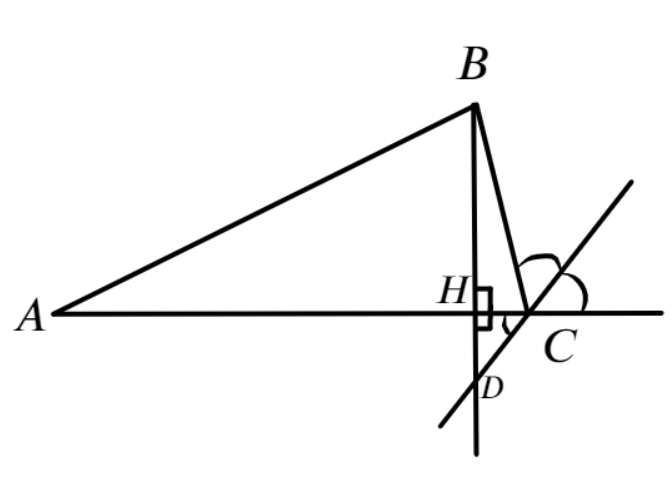
\includegraphics[scale=0.35]{g9-134.png}}
\end{figure}\\
Найдём $\angle C=180^\circ-80^\circ-24^\circ=76^\circ.$ Тогда внешний угол при вершине $C$ равен $180^\circ-76^\circ=104^\circ$ и угол $HCD$ равен его половине как вертикальный. Поэтому $\angle HDC=90^\circ-104^\circ:2=38^\circ.$
ewpage
oindent
